\documentclass{scrreprt}
\usepackage{listings}
\usepackage{underscore}
\usepackage[bookmarks=true]{hyperref}
\usepackage[utf8]{inputenc}
\usepackage[portuguese]{babel}
\hypersetup{
	bookmarks=false,    % show bookmarks bar?
	pdftitle={Software Requirement Specification},    % title
	pdfauthor={Jean-Philippe Eisenbarth},                     % author
	pdfsubject={TeX and LaTeX},                        % subject of the document
	pdfkeywords={TeX, LaTeX, graphics, images}, % list of keywords
	colorlinks=true,       % false: boxed links; true: colored links
	linkcolor=blue,       % color of internal links
	citecolor=black,       % color of links to bibliography
	filecolor=black,        % color of file links
	urlcolor=purple,        % color of external links
	linktoc=page            % only page is linked
}%
\def\myversion{1.0 }
\date{}
%\title
\usepackage{hyperref}
\usepackage{graphicx}
\usepackage{floatrow}

\usepackage{caption}
\usepackage{tocloft}

\newcommand{\listimagemname}{Lista de Imagens}
\newlistof{listofimagens}{img}{\listimagemname}

\newcommand{\listofimagenspage}{\listofimagens}

\renewcommand{\cftlistofimagenspresnum}{\listimagemname~}
\setlength{\cftlistofimagensnumwidth}{4em}

\begin{document}
	
	\begin{flushright}
		\rule{16cm}{5pt}\vskip1cm
		\begin{bfseries}
			\Huge{SOFTWARE REQUIREMENTS\\ SPECIFICATION}\\
			\vspace{0.8cm}
			for\\
			\vspace{0.8cm}
			App AgroLink\\
			
		\begin{figure}[h]
			\begin{minipage}{0.6\textwidth}
			\end{minipage}
			\hfill
			\begin{minipage}{0.3\textwidth}
				\centering
				
\includegraphics[width=\textwidth]{AGROLINK.png}
		
			\end{minipage}
		\end{figure}

			\LARGE{Version \myversion}\\
			\vspace{1cm}
			Prepared by : Nuno Nogueira (a2021156399)\\
			Paulo Gonçalves (a2020130672)\\
			Tiago Moita (a2021142357)\\
			\vspace{0.8cm}
			Submitted to : Projeto e Desenvolvimento Informático\\
			\vspace{0.8cm}
			\today\\
		\end{bfseries}
	\end{flushright}
	
	\tableofcontents
	
	\listoffigures
	
	\chapter{Introdução}
	
	\section{Objetivo }
	
	 O presente documento de especificação de requisitos de software enquadra-se no contexto da unidade currícular de Projeto e desenvolvimento Informático do terceiro ano da Licenciatura em Informática de Gestão. Será realizado o desenvolvimento de uma aplicação mobile para o setor agrícola, tendo como objetivo principal a simplificação de atividades rotineiras deste setor, podendo estas serem introduzidas num contexto virtual. Ao longo do documento, será realizada a especificação de requisitos, diagramas de casos de uso, diagrama de classes, os vários requisitos para o correto funcionamento desta aplicação e ainda alguns dos mockups base para uma simplificação do funcionamento desta aplicação mobile. Desta forma, será possível ter uma melhor compreensão da base inicial que dará fará de suporte à implementação deste aplicativo, possibilitanto um desenvolvimento mais rápido e ajustado ao produto final.
	
	\section{Convenções do Documento}
	
	Este documento foi estruturado de acordo com índice apresentado, por secções mais gerais e outras mais específicas, sendo algumas mais aprofundadas.
	No que diz respeito às propriedades do documento, este foi escrito no tipo de letra {\fontname\font}, com espaçamento simples, podendo apresentar alguma mudança nos títulos e subtítulos. Ao longo do trabalho especificam-se os requisitos a serem tidos em conta no desenvolvimento do sistema AgroLink,
	como base o modelo SRS (Software Requirements Specification) e com a ISO / IEC 12207 (norma associada aos processos do ciclo de vida de em software). Os requisitos estão estruturados de forma hierárquica, atribuindo-se uma prioridade em função de, quanto maior for o número de dígitos, maior será a 
	especificidade e simplicidade. A atribuição de prioridade a cada um dos requisitos permite resolver conflitos, gerir os mesmos da melhor forma e decidir sobre quais os requisitos 
	implementar.
	
	\section{Audiência pretendida e sugestões de leitura}
	
	A leitura e análise deste documento poderá ser do interesse de todos os utilizadores do sistema, tendo em conta o lugar que cada um ocupa dentro das organizações que decidirem implementar a sua utilização no dia a dia da empresa. Na fase inicial de utilização do sistema será importante que os principais dirigentes (direção e pessoal administrativo) acompanhem todo o processo de eventual transformação, atualização e manutenção, uma vez que são estes que diretamente podem interferir na sua utilização e apoiar outros utilizadores secundários (trabalhadores laborais).
	Apesar de considerarmos o documento de fácil leitura, consideramos que existem algumas partes mais relevantes para a maioria dos utilizadores, como é o caso da introdução e descrição geral, uma vez que a grande maioria dos utilizadores não necessitará de aceder a todas as propriedades do produto a ser desenvolvido. Todos os leitores deverão ler a Introdução (1) e a Descrição Geral (2), é imperativo que os gestores do software leiam todo o documento. A equipa de Direção necessita de conhecer o seu público-alvo e os programadores deverão ler todos os requisitos (4,5).
	
	
	\chapter{Descrição geral}
	
	\section{Perspetiva do produto}
	O presente projeto visa introduzir a aplicação AgroLink, uma ferramenta inovadora destinada a simplificar o dia a dia das pequenas e médias produções agrícolas. Com o objetivo de otimizar processos e melhorar os rendimentos das explorações, a AgroLink foi concebida para oferecer soluções práticas e acessíveis que atendam às necessidades específicas dos agricultores.
	Esta aplicação surge como resposta ao dia a dia exigente do setor agrícola que também este, permanece em constante evolução, onde a eficiência e a produtividade são fundamentais para o sucesso das empresas. Através deste sistema, os agricultores terão acesso a uma variedade de recursos e funcionalidades projetadas para simplificar tarefas diárias, como gestão de culturas, monitorizamento de condições climáticas, gestão de tarefas e visualização macro de toda a exploração.
	Além de proporcionar uma maior eficiência operacional, a AgroLink também visa promover a sustentabilidade e a inovação no setor agrícola, incentivando a práticas agrícolas responsáveis e facilitando o acesso a tecnologias avançadas.
	Tendo em vista o desenvolvimento qualificado deste sistema o seu desenvolvimento, guiar-se-à pelos seguintes parâmetros:
	\begin{itemize}
		\item Facilitar o acompanhamento e a gestão de culturas agrícolas;
		\item Fornecer informações atualizadas sobre as condições climáticas locais;
		\item Proporcionar uma visão macro de toda a exploração as atividades da exploração. 
	\end{itemize}
	De forma a compreender algumas das implementações mencionadas acima, apresenta-se a figura \ref{fig:diagramarelacional}, com as relações entre algumas classes do sistema. 
	
	\begin{figure}[!h]
		\centering
		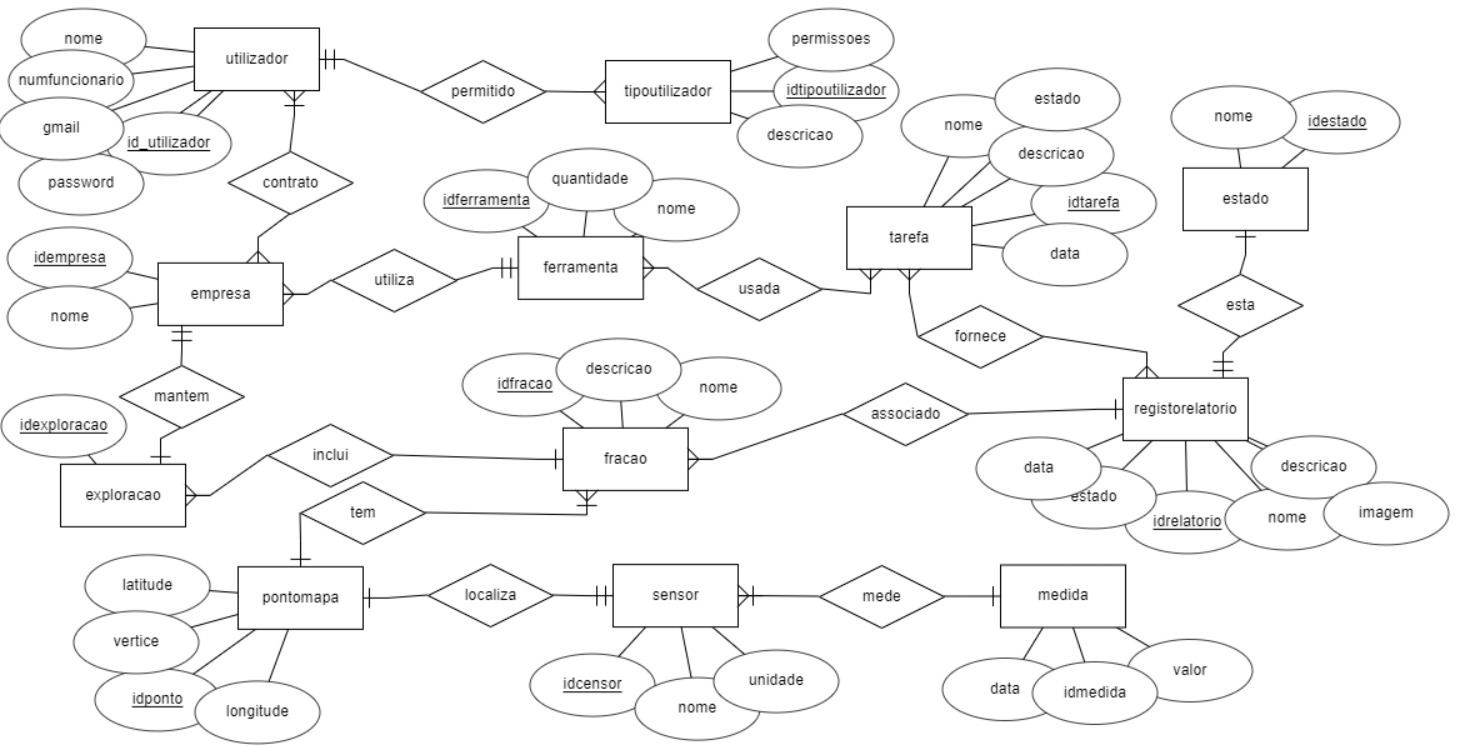
\includegraphics[width=0.9\linewidth]{DiagramaRelacional.png}
		\caption{Diagrama Relacional}
		\label{fig:diagramarelacional}
	\end{figure}

		
	\section{Características do Produto}
	Na utilização do sistema existem diferentes tipos de utilizadores (Trabalhador, Gestor da Produção e Administrador do Sistema) e consoante o utilizador existem também várias funcionalidades que podem ou não estar disponíveis, nomeadamente a criação, edição e remoção de objetos na base de dados. Algumas dessas características podem ser acedidas por todos e outras apenas são acedidas por utilizadores específicos.\\
	No seguimento da figura \ref{fig:diagramarelacional}, foi realizado o diagrama de classes que pode ser visto na figura \ref{fig:diagramadeclasses} onde se apresentão as princiapis classes do sistema e as suas ligações. 
	
	\begin{figure}[!h]
		\centering
		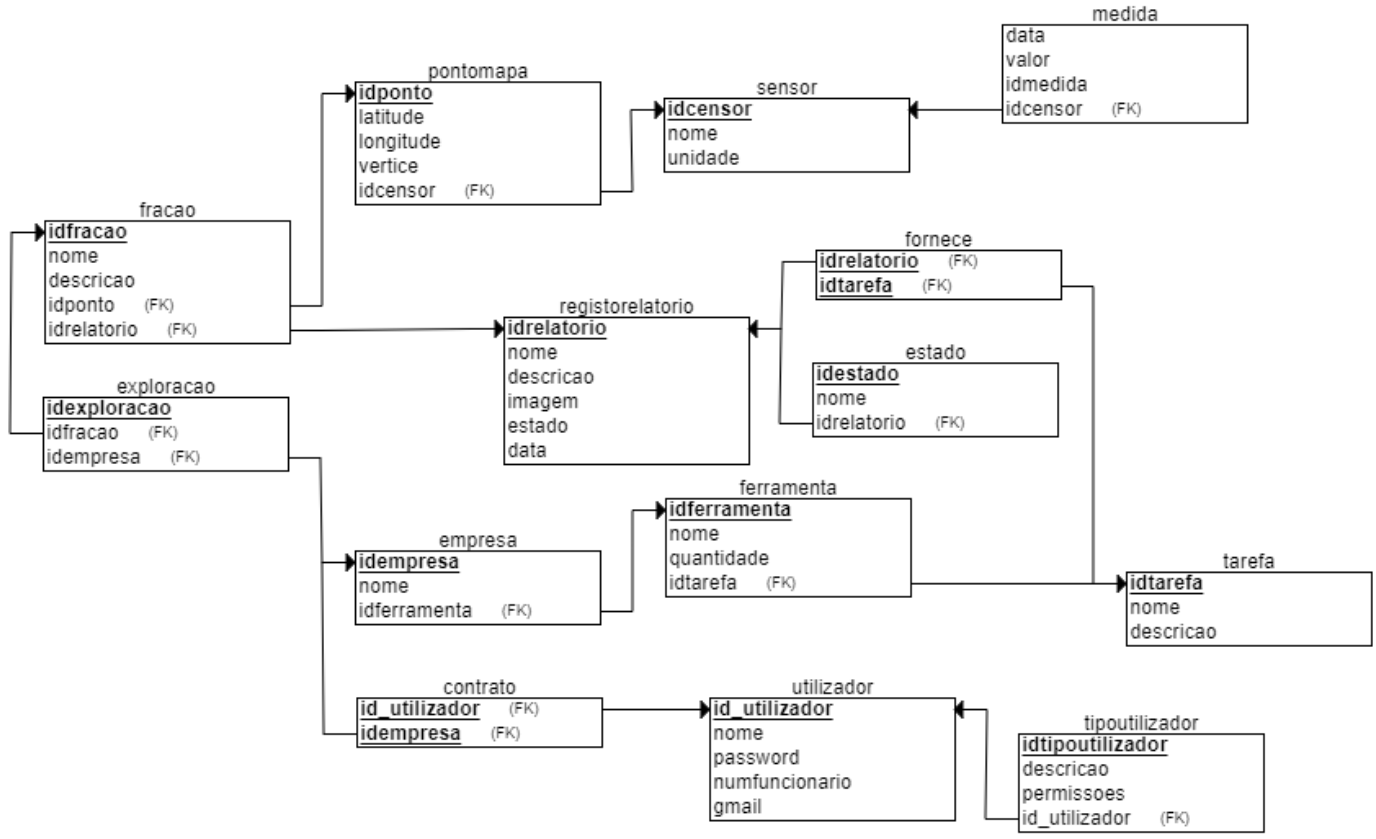
\includegraphics[width=0.7\linewidth]{DiagramaDeClasses.png}
		\caption{Diagrama de Classes}			\label{fig:diagramadeclasses}
	\end{figure}

	
	\section{Ambiente Operativo}
	
	Para o desenvolvimento do sistema atual, foram tidas em conta várias 
	plataformas existentes para que fosse possível toda a implementação e para que esta fosse realizada da melhor forma possível.
	\\ A aplicação deverá operar no sitema operativo Andriod e IOS uma vez que se trata de uma aplicação mobile e a linguagem de programação utilizada irá ser Python onde a plataforma de desenvolvimento será Beewave uma vez que permite o desenvolvimento nativo aplicacional. 
	\\Para a realização dos mockups foi utilizada a plataforma figma, que apresenta grande versatilidade e rápida aprendizagem na produção de designs.
	\\A construção dos diagramas, que permitem uma melhor compreensão de todo o funcionando do sistema, foi realizada no software visual paradigm. A figura \ref{fig:ambienteoperativo} apresenta todos os sistemas e aplicações que foram e irão ser utilizados ao longo de todo o desenvolvimento da aplicação Agrolink.
	
	
	\begin{figure}[!h]
		\centering
		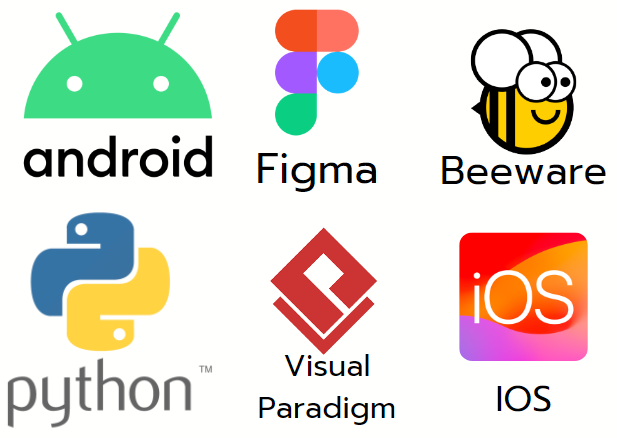
\includegraphics[width=0.3\linewidth]{AmbienteOperativo.png}
		\caption{Ambiente Operativo}
		\label{fig:ambienteoperativo}
	\end{figure}

	\section{Restrições de desenho e implementação}
	A aplicação AgroLink, pretende ser uma aplicação utilizada no contexto agrícola e com uma conecção permanente wifi de forma a permitir o acesso à sua base de dados, pelo que em algumas localizações dos terrenos poderá ser mais difícil o acesso imediato ao sistema, por questões de banda das telecomunicações.
	Será sempre tida em conta a importancia das precauções em relação ao 
	acesso e partilha de informação de qualquer utilizador do sistema, uma vez que com as novas políticas de proteção de dados associadas ao RGPD, condicionam a gestão da informação a partir dos dados pessoais. Neste caso é necessário prever a existência de protocolo de consentimento de divulgação de dados pessoais.
	Além disso, as passworks dos utilizadores serão criptografadas na base de dados, para garantir uma maior segurança dos utilizadores na base de dados.
		
		
		\chapter{ Características do Sistema}
	No sistema AgroLink existem três tipos de utilizadores: Trabalhador, Administrador do Sistema e Gestor da Produção.
	Os tópicos seguintes, clarifica as funcionalidades explicitas sobre a forma de 
	requisitos e ainda os casos de uso associados a cada tipo de utilizador e ainda alguns dos mockups do sistema, esclarecendo o leitor de como o sistema funciona e quais as características e particularidades desta aplicação. 
	A figura \ref{fig:appagrolink} apresenta a imagem da aplicação AgroLink nos dispositivos móveis onde este poderá ser instalado.
	
	\begin{figure}[h!]
		\centering
		
\includegraphics[width=0.2\linewidth]{AppAgrolink}
		\caption{App Agrolink}
		\label{fig:appagrolink}
	\end{figure}
	
	
	\section{Gestão de Utilizadores}
	Os requisitos funcionais deste sistema, como é o caso da Gestão de Utilizadores caracterizam-se pela possibilidade de manuseamento e alteração no sistema por parte de alguns utilizadores. A figura \ref{fig:Diagrama de-casos-de-uso---gestao-de-utilizadores} presente nos anexos, representa o diagrama de casos de uso para a gestão de 
	utilizadores, onde são representados todos os tipos de utiliadores do sistema.
		
		
	\subsection{Descrição e Prioridade}
	Todos os requisitos constituintes da gestão de utilizadores, têm Prioridade Alta. Estes requisitos constituem um papel fulcral no acesso à plataforma, assim como a quando da criação da empresa no sistema. Para ter acesso é necessário introduzir a empresa no sistema, criar um utilizador, procedimento que 
	poderá ser efetuado pelo Gestor da Produção e posteriormente também é possível adicionar mais utilizadores e realizar algumas alterações à informação dos 
	utilizadores.
	
	\subsection{Sequência de Resposta}
	Cada utilizador terá que de ter as suas próprias credencias, para poder aceder à sua conta. Será necessário criar conta para todos os utilizadores, no entanto, só será possível depois do gestor da produção criar a sua conta e a da empresa. A figura \ref{fig:mockupsgestaodeutilizadores} apresenta uma visão mais detalhada acerca dos casos de uso da Gestão de Utilizadores, "Efetuar Login", "Adicionar Empresa" e “Criar Utilizador”.
	
	\begin{figure}[!h]
		\centering
		\includegraphics[width=0.7\linewidth]{MockupsGestaoDeUtilizadores}
		\caption{Mockups - Gestão de Utilizadores}
		\label{fig:mockupsgestaodeutilizadores}
	\end{figure}
	
	\section{Gestão de Relatórios}
	A “Gestão de Relatórios" está associada à possibilidade de todos os utilizadores poderem interatuar com os relatórios gerados pelo gestor da produção, de forma a fazer um melhor rastreio das atividades realizadas na exploração. A figura \ref{fig:diagrama-de-casos-de-uso---gestao-de-relatorios} presente nos anexos, representa o diagrama de casos de uso para a gestão de relatórios.
	
	\subsection{Descrição e Prioridade}
	Uma vez que se trata de uma das principais características do sistema, grande parte dos requisitos são de alta prioridade, como a visualização de novas. A implementação desta área de gestão poderá ser importante para é fulcral para a organização das empresas já que conta com área de tarefas e de inserção de imagens.
	
	\subsection{Sequência de Resposta}
	Todos os utilizadores terão acesso à gestão de relatórios, assim como a possibilidade de os atualizarem. O gestor da produção deverá criar o ou os relatórios para cada fração e a partir desse momento ficará disponível para qualquer tipo de utilizador. A figura \ref{fig:mockupsgestaoderelatorios} apresenta uma visão mais detalhada acerca dos casos de uso da Gestão de Relatórios, "Adicionar Imagem", "Adicionar Tarefa", bem como outras outros casos de uso subjacentes.
	
	
	\begin{figure}[!h]
		\centering
		\includegraphics[width=0.5\linewidth]{MockupsGestaoDeRelatorios}
		\caption{Mockups - Gestão de Relatórios}
		\label{fig:mockupsgestaoderelatorios}
	\end{figure}
		
	\section{Gestão de Frações}
	A “Gestão de Frações", logo após da gestão de utilizadores, é a secção mais utilizada em todo o sistema, uma vez que esta incluí desde a adição das frações ao sistema, como também os sensores e é a base sobre a qual todas as informações estão associadas. Permite a adição  das frações ao mapa, assim como a sua visualização, a posterior associação de cada fração aos Relatórios. A figura \ref{fig:diagrama-de-casos-de-uso---gestao-de-fracoes} presente nos anexos, representa o diagrama de casos de uso para a gestão de frações.
	
	\subsection{Descrição e Prioridade}
	Uma vez que se trata de uma das principais características do sistema, grande parte dos requisitos são de alta prioridade, como a visualização de novas. A implementação desta área de gestão poderá ser importante para é fulcral para a organização das empresas já que conta com área de tarefas e de inserção de imagens.
	
	\subsection{Sequência de Resposta}
	Todos os utilizadores terão acesso à gestão de relatórios, assim como a possibilidade de os atualizarem. O gestor da produção deverá criar o ou os relatórios para cada fração e a partir desse momento ficará disponível para qualquer tipo de utilizador. A figura \ref{fig:mockupsgestaodefracoes}  apresenta uma visão mais detalhada acerca dos casos de uso da Gestão de Relatórios, "Adicionar Imagem", "Adicionar Tarefa", bem como outras outros casos de uso subjacentes.
	
	\begin{figure}[!h]
		\centering
		\includegraphics[width=0.5\linewidth]{MockupsGestaoDeFracoes.png}
		\caption{Mockups - Gestão de Frações}
		\label{fig:mockupsgestaodefracoes}
	\end{figure}
	
	\section{Gestão de Outras Operações}
	Na “Gestão de Outras Operações", constam várias funções que apesar de não serem as principais, complementam o bom uso da aplicação. Nesta secção, estão contemplados, os comunicados que podem ser adicionados pelo gestor da produção, os termos e condições que mantêm os utilizadores informados de como a aplicação opera em termos legais e ainda algumas outras formas de visualização dos menus principais. A figura \ref{fig:diagrama-de-casos-de-uso---gestao-de-outras-operacoes} apresenta uma visão mais detalhada acerca dos casos de uso da Gestão de Outras Operações.
	
	\subsection{Descrição e Prioridade}
	Nesta secção estão presentes algumas das características que não são fulcrais ao sistema, pelo que parte dos requisitos são de média e baixa prioridade. A implementação desta área de gestão poderá ser importante para é fulcral para a organização das empresas já que conta com área de tarefas e de inserção de imagens.
	
	\subsection{Sequência de Resposta}
	Todos os utilizadores terão acesso à gestão de relatórios, assim como a possibilidade de os atualizarem. O gestor da produção deverá criar o ou os relatórios para cada fração e a partir desse momento ficará disponível para qualquer tipo de utilizador. A figura \ref{fig:mockupsgestaodeoutrasoperacoes}  apresenta uma visão mais detalhada acerca dos casos de uso da Gestão de Relatórios, "Adicionar Imagem", "Adicionar Tarefa", bem como outras outros casos de uso subjacentes.
	
	\begin{figure}[!h]
		\centering
		\includegraphics[width=0.3\linewidth]{MockupsGestaoDeOutrasOperacoes}
		\caption{Mockups - Gestão de Outras Operações}
		\label{fig:mockupsgestaodeoutrasoperacoes}
	\end{figure}
	
	Para poder visualizar todas as relações este os mockups disponibilizados ao longo deste documento, deixamos o link do site onde formam criados os mockups do projeto \href{https://www.figma.com/file/64FxVuM0BBvMAQNQz9qsxQ/AgroLink---Mockups?type=design&mode=design&t=a60q5ceoFfV1y99Z-1}{www.figma.com/Projeto}.
	
	
	\chapter{Anexos}
	
	\section{Anexo A: Diagramas de Caso de Uso}
	
	\begin{figure}[!h]
		\centering
		\includegraphics[width=0.8\linewidth]{"Diagrama de Casos de Uso - Gestão de Utilizadores.png"}
		\caption{Diagrama de Casos de Uso - Gestão de Utilizadores}
		\label{fig:Diagrama de-casos-de-uso---gestao-de-utilizadores}
	\end{figure}
	
	\begin{figure}[!h]
		\centering
		\includegraphics[width=0.8\linewidth]{"Diagrama de Casos de Uso - Gestão de Relatórios.png"}
		\caption{Diagrama de Casos de Uso - Gestão de Relatórios}
		\label{fig:diagrama-de-casos-de-uso---gestao-de-relatorios}
	\end{figure}
	
	\begin{figure}[!h]
		\centering
		\includegraphics[width=0.8\linewidth]{"Diagrama de Casos de Uso - Gestão de Frações.png"}
		\caption{Diagrama de Casos de Uso - Gestão de Frações}
		\label{fig:diagrama-de-casos-de-uso---gestao-de-fracoes}
	\end{figure}
	
	\begin{figure}[!h]
		\centering
		\includegraphics[width=0.8\linewidth]{"Diagrama de Casos de Uso - Gestão de Outras Operações"}
		\caption{Diagrama de Casos de Uso - Gestão de Outras Operações}
		\label{fig:diagrama-de-casos-de-uso---gestao-de-outras-operacoes}
	\end{figure}
	
\end{document}